%+*** 111,112document.tex
% arara: indent: {overwrite: on, trace: on, localSettings: yes}
%===================================
%
%   Last edited: Hughes
%                11/18/12 (v9)
%
%===================================
\chapter{Logarithms}
\minitoc
\section{Logarithmic functions}
In our chapter on exponential functions we considered applications that 
lead to equations such as
\[
	10^x=19
\]
We can approximate solutions to such equations using graphical and 
numerical techniques. How can we solve these equations \emph{algebraically} 
though? The answer is to use \emph{logarithmic} functions.

\begin{pccdefinition}[The logarithm function]\label{log:def:logfunctions}
	The logarithmic function, base $b$, where $b>0$ and $b\ne 1$, is 
	defined by
	\[
		y=\log_b(x)
	\]
	if, and only if, 
	\[
		b^y=x
	\]
	The domain of the logarithmic function $y=\log_b(x)$ is $(0,\infty)$, and 
	the range is $(-\infty,\infty)$.
\end{pccdefinition}

\Cref{log:def:logfunctions} says that if we are given a \emph{logarithmic} 
expression then we can convert it into an equivalent \emph{exponential} 
expression. This is useful when evaluating logarithmic expressions.

%===================================
%   Author: Hughes
%   Date:   July 2012
%===================================
\begin{pccexample}
	Use a sentence to describe each of the following logarithmic expressions, and 
	then evaluate each expression
	\begin{multicols}{4}
		\begin{enumerate}
			\item $\log_2(32)$
			\item $\log_3(81)$
			\item $\log_5(25)$
			\item $\log_{73}(1)$
		\end{enumerate}
	\end{multicols}
	\begin{pccsolution}
		\begin{enumerate}
			\item The logarithm, base $2$, of $32$. In order to evaluate the expression, we need 
			to answer the question: what power do we raise $2$ to get $32$? The answer is $5$, so
			\[
				\log_2(32)=5
			\]
			\item The logarithm, base $3$, of $81$. What power do we raise $3$ to get $81$? The 
			answer is $4$, so
			\[
				\log_3(81)=4
			\]
			\item The logarithm, base $5$, of $25$. What power do we raise $5$ to get $25$? The 
			answer is $2$, so
			\[
				\log_5(25)=2
			\]
			\item The logarithm, base $73$, of $1$. We need to raise $73$ to the power $0$ 
			to get $1$, so
			\[
				\log_{73}(1)=0
			\]
		\end{enumerate}
	\end{pccsolution}
\end{pccexample}

%===================================
%   Author: Hughes
%   Date:   July 2012
%===================================
\begin{pccexample} 
	Convert each of the following exponential equations into their equivalent logarithm form
	\begin{multicols}{4}
		\begin{enumerate}
			\item $3^{5}=243$
			\item $7^{0}=1$
			\item $16^{\nicefrac{1}{2}}=4$
			\item $33^{-1}=\frac{1}{33}$
		\end{enumerate}
	\end{multicols}
	\begin{pccsolution}
		\begin{enumerate}
			\item $3^{5}=243$ is equivalent to 
			\[
				\log_3(243)=5
			\]
			\item $7^{0}=1$ is equivalent to 
			\[
				\log_7(1)=0
			\]
			\item $16^{\nicefrac{1}{2}}=4$ is equivalent to 
			\[
				\log_{16}(4)=\frac{1}{2}
			\]
			\item $33^{-1}=\frac{1}{33}$ is equivalent to
			\[
				\log_{33}\left( \frac{1}{33} \right)=-1
			\]
		\end{enumerate}
	\end{pccsolution}
\end{pccexample}
%===================================
%   Author: Hughes
%   Date:   July 2012
%===================================
\begin{pccexample}
	Convert each of the following logarithmic equations into their equivalent exponential form
	\begin{multicols}{4}
		\begin{enumerate}
			\item $\log_4\left( \frac{1}{4} \right)=-1$
			\item $\log_{6}(36)=2$
			\item $\log_{\frac{1}{2}}(4)=-2$
			\item $\log_{e}(e^8)=8$
		\end{enumerate}
	\end{multicols}
	\begin{pccsolution}
		\begin{enumerate}
			\item $\log_4\left( \frac{1}{4} \right)=-1$ is equivalent to
			\[
				4^{-1}=\frac{1}{4}
			\]
			\item $\log_{6}(36)=2$ is equivalent to
			\[
				6^2=36
			\]
			\item $\log_{\frac{1}{2}}(4)=-2$ is equivalent to 
			\[
				\left(\frac{1}{2}\right)^{-2}=4
			\]
			\item $\log_{e}(e^8)=8$ is equivalent to
			\[
				e^8=e^8
			\]
			In fact when evaluating a logarithm base $e$ we use a special notation, as we'll soon 
			see.
		\end{enumerate}
		\mbox{}
	\end{pccsolution}
\end{pccexample}

We have been able to perform all of our calculations so far using our knowledge of
arithmetic and exponents.  When faced with a 
logarithmic calculation that goes beyond this, we need to use a calculator
to compute the value. Most modern calculators can work in any base, 
but of all the possible choices that we have available there are  
two bases that are particularly important.

\begin{pccdefinition}[The common and natural logarithm functions]
	When working with logarithmic functions that have base $b$ and formula $y=\log_b(x)$,
	\begin{itemize}
		\item the \emph{common} logarithmic function has base $10$ and is 
		written as
		\[
			y=\log(x)
		\]
		\item the \emph{natural} logarithmic function has base $e$ and is
		written as
		\[
			y=\ln(x)
		\]
		It may help to recall from \vref{exp:def:e} that $e$ is called the \emph{natural} base.
	\end{itemize}
\end{pccdefinition}
%===================================
%   Author: Hughes
%   Date:   July 2012
%===================================
\begin{pccexample}[Domain]
	Find the domain of each the functions implied by the following formulas
	\begin{multicols}{2}
		\begin{enumerate}
			\item $f(x)=\log(x)$
			\item $g(x)=\log_3(2+x)$
			\item $h(x)=\ln(4x-5)$
			\item $j(x)=\log_7(x^2)$
		\end{enumerate}
	\end{multicols}
	\begin{pccsolution}
		\begin{enumerate}
			\item The domain of $f$ is $(0,\infty)$. Note that the base of $f$ is $10$; 
			$f$ is the common logarithmic function.
			\item To find the domain of $g$ we need to solve the inequality $2+x>0$. 
			The domain of $g$ is, therefore, $(-2,\infty)$.
			\item To find the domain of $h$ we need to solve the inequality $4x-5>0$.
			The domain of $h$ is $\left( \frac{5}{4},\infty \right)$. Note that the 
			base of $h$ is $e$; $h$ is the natural logarithmic function.
			\item To find the domain of $j$ we need to solve the inequality $x^2>0$. 
			The domain of $g$ is therefore $(-\infty,0)\cup (0,\infty)$.
		\end{enumerate}
	\end{pccsolution}
\end{pccexample}

One of the implications of \cref{log:def:logfunctions} is that there is 
a relationship between logarithmic functions and exponential functions. 
Explicitly, if $f$ is the exponential function that has formula
\[
	f(x)=b^x
\]
then the inverse function, $f^{-1}$, has formula
\[
	f^{-1}(x)=\log_b(x)
\]
We can use our knowledge of inverse functions (see \fixthis{insert vref reference to inverse function
section- doesn't exist yet!}) to help us graph logarithmic functions.

%===================================
%   Author: Hughes
%   Date:   July 2012
%===================================
\begin{pccexample}[Graphing]\label{log:ex:graphing}
	Use your knowledge of the function $f$ that has formula $f(x)=2^x$ 
	to help you graph its inverse function, $f^{-1}$, that has formula
	$f^{-1}(x)=\log_2(x)$.
	\begin{pccsolution}
		Let's start by constructing a table of values of the function $f$ in 
		\cref{log:tab:fandinverse}. We can easily construct a table of 
		values of $f^{-1}(x)$ by simply swapping the input and output values, 
		which we have done in \cref{log:tab:finverse}.
		
		\begin{table}[!htb]
			\renewcommand{\arraystretch}{1.25}
			\begin{minipage}{.5\textwidth}
				\centering
				\caption{$f$}
				\label{log:tab:fandinverse}
				\begin{tabular}{S[table-format=1.0]S[table-format=1.0]}
					\beforeheading 
					\heading{$x$} & \heading{$f(x)$} \\ \afterheading   
					\afterheading
					-3            & \num{1/8}        \\\normalline
					-2            & \num{1/4}        \\\normalline
					-1            & \num{1/2}        \\\normalline
					0             & 1                \\\normalline
					1             & 2                \\\normalline
					2             & 4                \\\normalline
					3             & 8                \\\lastline
				\end{tabular}
			\end{minipage}%
			\begin{minipage}{.5\textwidth}
				\centering
				\caption{$f^{-1}$}
				\label{log:tab:finverse}
				\begin{tabular}{S[table-format=1.0]S[table-format=1.0]}
					\beforeheading 
					\heading{$x$} & \heading{$f^{-1}(x)$} \\
					\afterheading
					\num{1/8}     & -3                    \\\normalline
					\num{1/4}     & -2                    \\\normalline
					\num{1/2}     & -1                    \\\normalline
					1             & 0                     \\\normalline
					2             & 1                     \\\normalline
					4             & 2                     \\\normalline
					8             & 3                     \\\lastline
				\end{tabular}
			\end{minipage}
		\end{table}
		
		If we plot the values we obtained in \cref{log:tab:fandinverse,log:tab:finverse} 
		and connect them using a smooth curve, then we obtain the curves given in \cref{log:fig:fandinverse}.
		\begin{figure}[!htb]
			\centering
			\begin{tikzpicture}
				\begin{axis}[
						xmin=-10,xmax=10,
						ymin=-10,ymax=10,
						width=.5\textwidth,
					]
					\addplot expression[domain=-10:3.32192]{2^x}node[axisnode,anchor=north west]{$y=2^x$};
					\addplot[soldot] coordinates{(-3,1/8)(-2,1/4)(-1,1/2)(0,1)(1,2)(2,4)(3,8)};
					\addplot[pccplot] expression[domain=0.001:10,samples=100]{ln(x)/ln(2)}node[axisnode,anchor=south east]{$y=\log_2(x)$};
					\addplot[soldot] coordinates{(1/8,-3)(1/4,-2)(1/2,-1)(1,0)(2,1)(4,2)(8,3)};
					\addplot[pccplot,dashed] expression[domain=-10:10]{x}node[axisnode,anchor=east,pos=0.2]{$y=x$};
				\end{axis}
			\end{tikzpicture}
			\caption{}
			\label{log:fig:fandinverse}
		\end{figure}
		
		There are a few more observations that we can make about $f$ and its inverse, using \cref{log:fig:fandinverse} 
		as a guide:
		\begin{itemize}
			\item the domain of $f$ is $(-\infty,\infty)$, and the range of $f$ is $(0,\infty)$; this means
			that the domain of $f^{-1}$ is $(0,\infty)$, and the range of $f^{-1}$ is $(-\infty,\infty)$;
			\item the function $f$ has a \emph{horizontal} asymptote with equation $y=0$; this necessarily
			means that the function $f^{-1}$ has a \emph{vertical} asymptote with equation $x=0$;
			\item the function $f$ does not have a \emph{vertical} asymptote| this therefore
			implies that the function $f^{-1}$ does not have a \emph{horizontal} asymptote;
			\item the curves of $f$ and $f^{-1}$ are symmetric about the line $y=x$.
		\end{itemize}
	\end{pccsolution}
\end{pccexample}


\begin{doyouunderstand}
	\begin{problem}
	Repeat \cref{log:ex:graphing} using the function $f$ that has formula $f(x)=3^x$.
	\begin{shortsolution}
		\begin{tabular}[t]{S[table-format=1.0]S[table-format=2.0]}
			\beforeheading 
			\heading{$x$} & \heading{$f(x)$} \\
			\afterheading
			-3            & \num{1/27}       \\\normalline
			-2            & \num{1/9}        \\\normalline
			-1            & \num{1/3}        \\\normalline
			0             & 1                \\\normalline
			1             & 3                \\\normalline
			2             & 9                \\\normalline
			3             & 27               \\\lastline
		\end{tabular}
				
		\begin{tabular}{S[table-format=1.0]S[table-format=1.0]}
			\beforeheading 
			\heading{$x$} & \heading{$f^{-1}(x)$} \\
			\afterheading
			\num{1/27}    & -3                    \\\normalline
			\num{1/9}     & -2                    \\\normalline
			\num{1/3}     & -1                    \\\normalline
			1             & 0                     \\\normalline
			3             & 1                     \\\normalline
			9             & 2                     \\\normalline
			27            & 3                     \\\lastline
		\end{tabular}
				
		\begin{tikzpicture}
			\begin{axis}[
					xmin=-5,xmax=5,
					ymin=-30,ymax=30,
				]
				\addplot expression[domain=-5:3.0959]{3^x}node[axisnode,anchor=north west]{$y=3^x$};
				\addplot[soldot] coordinates{(-3,1/27)(-2,1/9)(-1,1/3)(0,1)(1,3)(2,9)(3,27)};
				\addplot[pccplot] expression[domain=0.0000000001:5,samples=100]{ln(x)/ln(3)}node[axisnode,pos=0,anchor=south west]{$y=\log_3(x)$};
				\addplot[soldot] coordinates{(1/27,-3)(1/9,-2)(1/3,-1)(1,0)(3,1)(9,2)(27,3)};
			\end{axis}
		\end{tikzpicture}
	\end{shortsolution}
	\end{problem}
\end{doyouunderstand}

There is a strong relationship between the logarithmic function $f$ that has formula
$f(x)=\log_b(x)$ and its inverse exponential function $f^{-1}$ that has formula
$f^{-1}(x)=b^x$. We can think of both functions as a type of \emph{mapping} from
their domains to their respective ranges. There are many possible ways to visualize
the mapping| one such image is shown in \cref{log:fig:mapping}. Notice that
the mapping lends itself well to highlighting \cref{log:prop:inv1,log:prop:inv2}, 
which detail the composition of logarithmic and exponential functions
\[
	(f\circ f^{-1})(x)=(f^{-1}\circ f)(x)=x
\]

\begin{figure}[!htb]
	\centering
	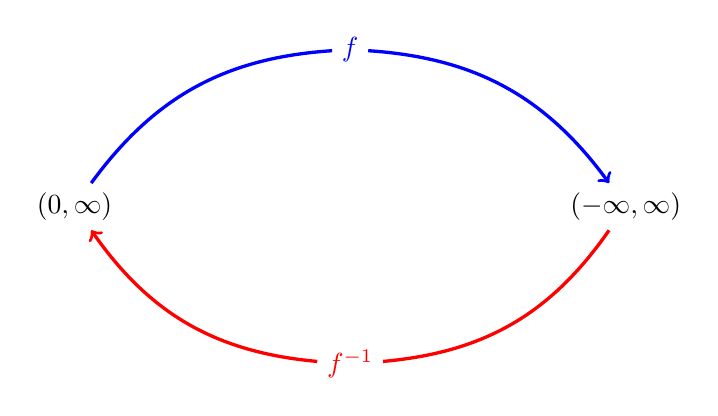
\begin{tikzpicture}
		% set up nodes
		\node (domain) at (0,0){$(0,\infty)$};
		\node (range) at (7,0){$(-\infty,\infty)$};
		\node[text=blue] (f) at (3.5,2) {$f$};
		\node[text=red] (finv) at (3.5,-2) {$f^{-1}$};
		% connect them
		\draw[blue,very thick] (domain) to[bend left=25] (f);
		\draw[->,very thick,blue] (f) to[bend left=25] (range);
		\draw[red,very thick] (range) to[bend left=25] (finv);
		\draw[->,red,very thick] (finv) to[bend left=25] (domain);
	\end{tikzpicture}
	\caption{Visualizing the mappings of $f$ and $f^{-1}$, where $f$ 
		has formula $f(x)=\log_b(x)$ and $f^{-1}$ has formula $f^{-1}(x)=b^x$.}
	\label{log:fig:mapping}
\end{figure}

Our examples so far have concentrated on familiarizing ourselves
with logarithmic functions but we have yet to see an application. 
The logarithmic functions have a myriad of applications| in particular, 
they can be used to help us study examples  that otherwise could 
only be attempted from a graphical or numerical perpesctive.

%===================================
%   Author: Hughes
%   Date:   July 2012
%===================================
\begin{pccexample}
	The number of radioactive atoms in a sample of Carbon-14 decays according to the model
	\[
		Q(t)= Q_0\,e^{-0.000120968t},
	\]
	where $Q_0$ is the initial mass of the radioactive atoms and $Q(t)$ is the mass of radioactive atoms $t$ years after the sample was established.
	
	What is the half-life of the sample?
	\begin{pccsolution}
		We need to find the value of $t$ that satisfies the equation $Q(t)=\frac{Q_0}{2}$. 
		We proceed using the following steps
		\begin{align*}
			\frac{Q_0}{2}=Q_0\,e^{-0.000120968t} & \Rightarrow \frac{1}{2}=e^{-0.000120968t}                            \\
			                                     & \Rightarrow \ln\left( \frac{1}{2} \right) = -0.000120968t            \\
			                                     & \Rightarrow t = -\frac{1}{-0.000120968}\ln\left( \frac{1}{2} \right) \\
			                                     & \phantom{ {}\Rightarrow t} = 5370                                    
		\end{align*}
		We conclude that the half-life of the sample is $5370$ years.
	\end{pccsolution}
\end{pccexample}

%===================================
%   Author: Neft (Hughes)
%   Date:   August 2012
%===================================
\begin{pccexample}[The RC circuit]
	A \emph{capacitor} is a device that stores electrical energy in the form of charged particles.
	The \emph{voltage} on the capacitor is a result of the electric field created by the particles and
	is proportional to the amount of charge stored. A \emph{resistor} is a device that dissipates
	electrical energy. If a capacitor is charged up and then connected across a resistor, the
	capacitor discharges and the voltage drops.
	
	The voltage (in \si{\volt}), on the capacitor as it is being discharged is modeled by the
	function $V$ that has formula 
	\[
		V(t)=V_0e^{-\frac{t}{RC}}
	\]
	where $V_0$ is the initial capacitor voltage, $R$ is the value of the
	resistor (in \si{\ohm}), $C$ is the value of the capacitor (in \si{\farad}) and $t$ is time (in \si{\second}).
	\begin{enumerate}
		\item Suppose that a $1.0\times 10^{-6}$-farad capacitor, initially charged to 
		$\SI{12}{\volt}$, is connected across a $\SI{10,000}{\ohm}$-resistor. 
		How long will it take for the voltage on the capacitor to drop to half 
		of its original value?
		\item Suppose the capacitor is initially charged to $\SI{20}{\volt}$. How long
		will it take for the voltage to drop to one half of its original value?
		\item Suppose the capacitor is initially charged up to $\SI{100}{\volt}$. How 
		long will it take for the voltage to drop to one half of its original value?
		\item What effect will doubling the \emph{resistance} have on the time it takes for the voltage to
		drop to one half of its initial value?
	\end{enumerate}
	\begin{pccsolution}
		\begin{enumerate}
			\item We need to solve the equation $\frac{1}{2}V_0=V_0e^{-\frac{t}{RC}}$:
			\begin{align*}
				6 = 12 e^{-100t} & \Rightarrow \frac{1}{2}=e^{-100t}                       \\
				                 & \Rightarrow \ln\left(\frac{1}{2}\right)=-100t           \\
				                 & \Rightarrow t=-\frac{1}{100}\ln\left(\frac{1}{2}\right) \\
				                 & \phantom{ {}\Rightarrow t}\approx 0.007                 
			\end{align*}
			It takes about $\SI{0.007}{\second}$ for the voltage of the capacitor to 
			reach one half of its initial value.
			\item We need to solve the equation $\frac{1}{2}V_0=V_0e^{-\frac{t}{RC}}$:
			\begin{align*}
				10 = 20 e^{-100t} & \Rightarrow \frac{1}{2}=e^{-100t}                       \\
				                  & \Rightarrow \ln\left(\frac{1}{2}\right)=-100t           \\
				                  & \Rightarrow t=-\frac{1}{100}\ln\left(\frac{1}{2}\right) \\
				                  & \phantom{ {}\Rightarrow t}\approx 0.007                 
			\end{align*}
			It takes about $\SI{0.007}{\second}$ for the voltage of the capacitor to 
			reach one half of its initial value. Does this sound familiar?
			\item We need to solve the equation $\frac{1}{2}V_0=V_0e^{-\frac{t}{RC}}$:
			\begin{align*}
				50 = 100 e^{-100t} & \Rightarrow \frac{1}{2}=e^{-100t}                       \\
				                   & \Rightarrow \ln\left(\frac{1}{2}\right)=-100t           \\
				                   & \Rightarrow t=-\frac{1}{100}\ln\left(\frac{1}{2}\right) \\
				                   & \phantom{ {}\Rightarrow t}\approx 0.007                 
			\end{align*}
			It takes about $\SI{0.007}{\second}$ for the voltage of the capacitor to 
			reach one half of its initial value. There seems to be a pattern here\ldots
			\item If we double the resistance to $\SI{20,000}{\ohm}$ then we need 
			to solve the equation $\frac{1}{2}V_0=V_0e^{-50t}$; note that the value of $V_0$
			does not affect our calculations
			\begin{align*}
				\frac{1}{2}V_0 = V_0 e^{-50t} & \Rightarrow \frac{1}{2}=e^{-50t}                       \\
				                              & \Rightarrow \ln\left(\frac{1}{2}\right)=-50t           \\
				                              & \Rightarrow t=-\frac{1}{50}\ln\left(\frac{1}{2}\right) \\
				                              & \phantom{ {}\Rightarrow t}\approx 0.014                
			\end{align*}
			We conclude that doubling the resistance doubles the time  it takes (to about $\SI{0.014}{\second}$) 
			for the voltage on the capacitor to reach half of its initial value.
		\end{enumerate}
	\end{pccsolution}
\end{pccexample}


\begin{exercises}
%===================================
%   Author: Hughes
%   Date:   July 2012
%===================================
\begin{problem}[Domain]
Find the domain of each of the functions implied by the following formulas. 
\begin{multicols}{4}
	\begin{subproblem}
		$f(x)=\log_4(x+7)$ 
		\begin{shortsolution}
			$(-7,\infty)$
		\end{shortsolution}
	\end{subproblem}
	\begin{subproblem}
		$g(x)=\log_9(x-2)$ 
		\begin{shortsolution}
			$(2,\infty)$
		\end{shortsolution}
	\end{subproblem}
	\begin{subproblem}
		$h(x)=5\log(3x)$ 
		\begin{shortsolution}
			$(0,\infty)$
		\end{shortsolution}
	\end{subproblem}
	\begin{subproblem}
		$j(x)=8-\log_2(4x+3)$ 
		\begin{shortsolution}
			$\left( -\frac{3}{4},\infty \right)$
		\end{shortsolution}
	\end{subproblem}
	\begin{subproblem}
		$k(x)=\log_6(x^2-9)$ 
		\begin{shortsolution}
			$(-\infty,-3)\cup (3,\infty)$
		\end{shortsolution}
	\end{subproblem}
	\begin{subproblem}
		$l(x)=3\log_8(4-2x^2)$ 
		\begin{shortsolution}
			$(-\sqrt{2},\sqrt{2})$
		\end{shortsolution}
	\end{subproblem}
	\begin{subproblem}
		$m(x)=\ln(2^x)$ 
		\begin{shortsolution}
			$(-\infty,\infty)$
		\end{shortsolution}
	\end{subproblem}
	\begin{subproblem}
		$n(x)=2^{\log(x)}$ 
		\begin{shortsolution}
			$(0,\infty)$
		\end{shortsolution}
	\end{subproblem}
\end{multicols}
\end{problem}
%===================================
%   Author: Hughes
%   Date:   July 2012
%===================================
\begin{problem}[Transformations: given the formula, describe the transformation]
Describe each of the functions $g$, $h$, $j$, and $k$ in terms of transformations 
of the logarithmic function $f$ that has formula $f(x)=\log(x)$. State the domain 
of each function.
\begin{multicols}{4}
	\begin{subproblem}
		$g(x)=\log(x+3)$ 
		\begin{shortsolution}
			$g$ is the function $f$ shifted to the left by $3$ units. The domain
			of $g$ is $(-3,\infty)$.
		\end{shortsolution}
	\end{subproblem}
	\begin{subproblem}
		$h(x)=\log(x-5)$ 
		\begin{shortsolution}
			$h$ is the function $f$ shifted to the right by $5$ units. The domain
			of $h$ is $(5,\infty)$.
		\end{shortsolution}
	\end{subproblem}
	\begin{subproblem}
		$j(x)=\log(2(x+7))$ 
		\begin{shortsolution}
			$j$ is the function $f$ horizontally compressed by a factor of $2$, 
			and shifted to the left by $7$ units. The domain of $j$ is $(-7,\infty)$.
		\end{shortsolution}
	\end{subproblem}
	\begin{subproblem}
		$k(x)=5\log(-x)$ 
		\begin{shortsolution}
			$k$ is the function $f$ reflected across the vertical axis, and vertically
			stretched by a factor of $5$. The domain of $k$ is $(-\infty,0)$.
		\end{shortsolution}
	\end{subproblem}
\end{multicols}
\end{problem}

%===================================
%   Author: Hughes
%   Date:   July 2012
%===================================
\begin{problem}[Transformations: given the transformation, find the formula]
Let $f$ be the function that has formula $f(x)=\log(x)$. In each of the following 
problems apply the given transformation to the function $f$ and 
write a formula for the transformed version of $f$.
\begin{multicols}{2}
	\begin{subproblem}
		Shift $f$ to the right by $2$ units. 
		\begin{shortsolution}
			$f(x-2)=\log(x-2)$
		\end{shortsolution}
	\end{subproblem}
	\begin{subproblem}
		Shift $f$ to the left by $5$ units. 
		\begin{shortsolution}
			$f(x+5)=\log(x+5)$
		\end{shortsolution}
	\end{subproblem}
	\begin{subproblem}
		Shift $f$ up by 11 units. 
		\begin{shortsolution}
			$f(x)+11=\log(x)+11$
		\end{shortsolution}
	\end{subproblem}
	\begin{subproblem}
		Shift $f$ down by 1 unit. 
		\begin{shortsolution}
			$f(x)-1=\log(x)-1$
		\end{shortsolution}
	\end{subproblem}
\end{multicols}
\end{problem}

%===================================
%   Author: Hughes
%   Date:   July 2012
%===================================
\begin{problem}[Find the base from graphs]\label{log:prob:findbase}
Consider the functions graphed in \cref{log:fig:findbase}. Each function 
has a formula of the form $y=\log_b(x+a)$, where $b$ is the base, and 
$a$ is given for each function. Use the ordered pair given in each graph to find the base, $b$.
\begin{shortsolution}
	\begin{itemize}
		\item \Vref{log:fig:findbase1}: $b=2$, so $y=\log_2(x)$;
		\item \Vref{log:fig:findbase2}: $b=4$, so $y=\log_4(x+3)$;
		\item \Vref{log:fig:findbase3}: $b=\frac{1}{2}$, so $y=\log_{\frac{1}{2}}(x-4)$;
		\item \Vref{log:fig:findbase4}: $b=\frac{1}{3}$, so $y=\log_{\frac{1}{3}}(x+2)$.
	\end{itemize}
\end{shortsolution}

\begin{figure}[htb]
	\begin{widepage}
	\begin{subfigure}{.2\textwidth}
		\centering
		\begin{tikzpicture}
			\begin{axis}[
					framed,
					minor xtick={-8,-4,4,8},
					xtick={-4},
					minor ytick={-8,-4,4,8},
					ytick={4},
					grid=both,
					xmin=-10,xmax=10,
					ymin=-10,ymax=10,
				]
				\addplot expression[domain=0.001:10,samples=50]{ln(x)/ln(2)};
				\addplot[soldot]coordinates{(8,3)}node[axisnode,anchor=south]{$(8,3)$};
			\end{axis}
		\end{tikzpicture}
		\caption{$y=\log_b(x)$}
		\label{log:fig:findbase1}
	\end{subfigure}%
	\hfill
	\begin{subfigure}{.2\textwidth}
		\centering
		\begin{tikzpicture}
			\begin{axis}[
					framed,
					minor xtick={-8,-4,4,8},
					xtick={4},
					minor ytick={-8,-4,4,8},
					ytick={-4},
					grid=both,
					xmin=-10,xmax=10,
					ymin=-10,ymax=10,
				]
				\addplot expression[domain=-2.999999:10,samples=100]{ln(x+3)/ln(4)};
				\addplot[soldot]coordinates{(-1,1/2)}node[axisnode,anchor=south east]{$\left(-1,\frac{1}{2}\right)$};
			\end{axis}
		\end{tikzpicture}
		\caption{$y=\log_b(x+3)$}
		\label{log:fig:findbase2}
	\end{subfigure}%
	\hfill
	\begin{subfigure}{.2\textwidth}
		\centering
		\begin{tikzpicture}
			\begin{axis}[
					framed,
					minor xtick={-8,-4,4,8},
					xtick={-4},
					minor ytick={-8,-4,4,8},
					ytick={4},
					grid=both,
					xmin=-10,xmax=10,
					ymin=-10,ymax=10,
				]
				\addplot expression[domain=4.001:10,samples=50]{ln(x-4)/ln(1/2)};
				\addplot[soldot]coordinates{(6,-1)}node[axisnode,anchor=north]{$(6,-1)$};
			\end{axis}
		\end{tikzpicture}
		\caption{$y=\log_b(x-4)$}
		\label{log:fig:findbase3}
	\end{subfigure}%
	\hfill
	\begin{subfigure}{.2\textwidth}
		\centering
		\begin{tikzpicture}
			\begin{axis}[
					framed,
					minor xtick={-8,-4,4,8},
					xtick={-4},
					minor ytick={-8,-4,4,8},
					ytick={-4},
					grid=both,
					xmin=-10,xmax=10,
					ymin=-10,ymax=10,
				]
				\addplot expression[domain=-1.99997:10,samples=100]{ln(x+2)/ln(1/3)};
				\addplot[soldot]coordinates{(7,-2)}node[axisnode,anchor=north]{$(7,-2)$};
			\end{axis}
		\end{tikzpicture}
		\caption{$y=\log_b(x+2)$}
		\label{log:fig:findbase4}
	\end{subfigure}%
	\caption{Graphs for \cref{log:prob:findbase}}
	\label{log:fig:findbase}
	\end{widepage}
\end{figure} 
\end{problem}

%===================================
%   Author: Hughes
%   Date:   July 2012
%===================================
\begin{problem}[Solving exponential equations with base $10$ and base $e$]
Use \cref{log:def:logfunctions} to solve each of the following equations. Give both 
the exact and an approximate solution.
\begin{multicols}{4}
	\begin{subproblem}
		$e^x=7$ 
		\begin{shortsolution}
			$x=\ln(7)\approx 1.95$
		\end{shortsolution}
	\end{subproblem}
	\begin{subproblem}
		$e^x+5=10$ 
		\begin{shortsolution}
			$x=\ln(5)\approx 1.61$
		\end{shortsolution}
	\end{subproblem}
	\begin{subproblem}
		$e^{x+5}=10$  
		\begin{shortsolution}
			$x=\ln(10)-5\approx -2.70$
		\end{shortsolution}
	\end{subproblem}
	\begin{subproblem}
		$e^{5x+7}-4=2$ 
		\begin{shortsolution}
			$x=\frac{1}{5}(\ln(6)-7)\approx -1.04$
		\end{shortsolution}
	\end{subproblem}
	\begin{subproblem}
		$10^x=1$ 
		\begin{shortsolution}
			$x=0$
		\end{shortsolution}
	\end{subproblem}
	\begin{subproblem}
		$10^{x+1}=11$ 
		\begin{shortsolution}
			$x=\log(11)-1\approx 0.04$
		\end{shortsolution}
	\end{subproblem}
	\begin{subproblem}
		$10^{2x}=4$ 
		\begin{shortsolution}
			$x=\frac{\log(4)}{2}\approx 0.30$
		\end{shortsolution}
	\end{subproblem}
	\begin{subproblem}
		$10^{4-x}=21$ 
		\begin{shortsolution}
			$x=4-\log(21)\approx 2.68$
		\end{shortsolution}
	\end{subproblem}
	\begin{subproblem}
		$5e^{2x}+1=10$ 
		\begin{shortsolution}
			$x=\frac{1}{2}\ln\left( \frac{9}{5} \right)\approx 0.29$
		\end{shortsolution}
	\end{subproblem}
	\begin{subproblem}
		$8-7e^{-3x}=-10$ 
		\begin{shortsolution}
			$x=-\frac{1}{3}\ln\left( \frac{18}{7} \right)\approx -0.31$
		\end{shortsolution}
	\end{subproblem}
	\begin{subproblem}
		$9e^{5-x}-1=0$ 
		\begin{shortsolution}
			$x=5-\ln\left( \frac{1}{9} \right)\approx 7.20$
		\end{shortsolution}
	\end{subproblem}
	\begin{subproblem}
		$e^{3x}-4=-5e^{3x}$ 
		\begin{shortsolution}
			$x=\frac{1}{3}\ln\left( \frac{2}{3} \right)\approx -0.14$
		\end{shortsolution}
	\end{subproblem}
\end{multicols}
\end{problem}

%===================================
%   Author: Hughes
%   Date:   July 2012
%===================================
\begin{problem}[Solving logarithmic equations with base $10$ and base $e$]
Use \cref{log:def:logfunctions} to solve each of the following equations. Give both 
the exact and an approximate solution.
\begin{multicols}{4}
	\begin{subproblem}
		$\ln(x)=7$ 
		\begin{shortsolution}
			$x=e^7\approx 1096.63$
		\end{shortsolution}
	\end{subproblem}
	\begin{subproblem}
		$2\ln(x)=-3$ 
		\begin{shortsolution}
			$x=e^{-\nicefrac{3}{2}}\approx 0.22$
		\end{shortsolution}
	\end{subproblem}
	\begin{subproblem}
		$5-4\ln(2x)=13$ 
		\begin{shortsolution}
			$x=\frac{e^{-2}}{2}\approx 0.07$
		\end{shortsolution}
	\end{subproblem}
	\begin{subproblem}
		$(\ln(x))^2=5$ 
		\begin{shortsolution}
			$x=e^{\sqrt{5}}\approx 9.36$ and $x=e^{-\sqrt{5}}\approx 0.11$
		\end{shortsolution}
	\end{subproblem}
	\begin{subproblem}
		$\log(x)=7$ 
		\begin{shortsolution}
			$x=10^7$
		\end{shortsolution}
	\end{subproblem}
	\begin{subproblem}
		$3-\log(x)=0$ 
		\begin{shortsolution}
			$x=1000$
		\end{shortsolution}
	\end{subproblem}
	\begin{subproblem}
		$\log(5x+2)=-3$ 
		\begin{shortsolution}
			$x=\frac{1}{5}\left( 10^{-3}-2 \right)\approx -0.40$
		\end{shortsolution}
	\end{subproblem}
	\begin{subproblem}
		$\log(5-x)=\log_2(8)$ 
		\begin{shortsolution}
			$x=-995$
		\end{shortsolution}
	\end{subproblem}
\end{multicols}
\end{problem}


%===================================
%   Author: Hughes
%   Date:   July 2012
%===================================
\begin{problem}[Find the base from tables]\label{log:prob:findbasetabs}
\Crefrange{log:tab:findbase1}{log:tab:findbase4} show values of four 
different functions; each function has the form $y=\log_b(ax)$ where
$b$ is the base, and $a$ is given for each function. 
Use any ordered pair you wish from each table to find the base, $b$, 
for each function.
\begin{shortsolution}
	\begin{itemize}
		\item \Vref{log:tab:findbase1}: $b=2$, so $y=\log_2(3x)$;
		\item \Vref{log:tab:findbase2}: $b=3$, so $y=\log_3(5x)$;
		\item \Vref{log:tab:findbase3}: $b=\frac{1}{4}$, so $y=\log_{\frac{1}{4}}(x)$;
		\item \Vref{log:tab:findbase4}: $b=\frac{1}{3}$, so $y=\log_{\frac{2}{3}}(-2x)$.
	\end{itemize}
\end{shortsolution}

\end{problem}
\begin{table}[htb]
	\renewcommand{\arraystretch}{1.25}
	\begin{widepage}
	\caption{Tables for \cref{log:prob:findbasetabs}}
	\label{log:tab:findbase}
	\begin{subtable}{.2\textwidth}
		\centering
		\caption{$y=\log_b(3x)$}
		\label{log:tab:findbase1}
		\begin{tabular}{S[table-format=1.0]S[table-format=1.0]}
			\beforeheading 
			\heading{$x$} & \heading{$y$} \\
			\afterheading
			\num{1/16}    & 1             \\  \normalline
			\num{1/3}     & 0             \\  \normalline
			\num{2/3}     & 1             \\  \normalline
			\num{4/3}     & 2             \\  \normalline
			\num{8/3}     & 3             \\  \lastline
		\end{tabular}
	\end{subtable}%
	\hfill
	\begin{subtable}{.2\textwidth}
		\centering
		\caption{$y=\log_b(5x)$}
		\label{log:tab:findbase2}
		\begin{tabular}{S[table-format=1.0]S[table-format=1.0]}
			\beforeheading 
			\heading{$x$} & \heading{$y$} \\
			\afterheading
			\num{1/135}   & -3            \\  \normalline
			\num{1/45}    & -2            \\  \normalline
			\num{1/15}    & -1            \\  \normalline
			\num{1/5}     & 0             \\  \normalline
			\num{3/5}     & 1             \\  \lastline
		\end{tabular}
	\end{subtable}%
	\hfill
	\begin{subtable}{.2\textwidth}
		\centering
		\caption{$y=\log_b(x)$}
		\label{log:tab:findbase3}
		\begin{tabular}{S[table-format=1.0]S[table-format=1.0]}
			\beforeheading 
			\heading{$x$} & \heading{$y$} \\
			\afterheading
			16            & -2            \\  \normalline
			4             & -1            \\  \normalline
			1             & 0             \\  \normalline
			\num{1/4}     & 1             \\  \normalline
			\num{1/16}    & 2             \\  \lastline
		\end{tabular}
	\end{subtable}%
	\hfill
	\begin{subtable}{.2\textwidth}
		\centering
		\caption{$y=\log_b(-2x)$}
		\label{log:tab:findbase4}
		\begin{tabular}{S[table-format=1.0]S[table-format=1.0]}
			\beforeheading 
			\heading{$x$} & \heading{$y$} \\
			\afterheading
			\num{-9/8}    & -2            \\  \normalline
			\num{-3/4}    & -1            \\  \normalline
			-1            & 0             \\  \normalline
			\num{-1/3}    & 1             \\  \normalline
			\num{-2/9}    & 2             \\  \lastline
		\end{tabular}
	\end{subtable}%
	\end{widepage}
\end{table} 


%===================================
%   Author: Hughes
%   Date:   July 2012
%===================================
\begin{problem}[Inverse functions]
Let $f$ be the function that has formula $f(x)=4^x$. 
\begin{subproblem}\label{log:prob:invconstruct}
	Construct a table of values of $f$, allowing $x$ to take integer values on the interval $[-3,3]$.
	\begin{shortsolution}
		\begin{tabular}[t]{S[table-format=1.0]S[table-format=1.0]}
			\beforeheading
			\heading{$x$} & \heading{$f(x)$} \\
			\afterheading
			-3            & \num{1/64}       \\\normalline
			-2            & \num{1/16}       \\\normalline
			-1            & \num{1/4}        \\\normalline
			0             & 1                \\\normalline
			1             & 4                \\\normalline
			2             & 16               \\\normalline
			3             & 64               \\\lastline
		\end{tabular}
	\end{shortsolution}
\end{subproblem}
\begin{subproblem}\label{log:prob:invconstructuse}
	Use your answer to \cref{log:prob:invconstruct} to construct a table of values 
	of the function $f^{-1}$.
	\begin{shortsolution}
		\begin{tabular}[t]{S[table-format=1.0]S[table-format=1.0]}
			\beforeheading
			\heading{$x$} & \heading{$f^{-1}(x)$} \\
			\afterheading
			\num{1/64}    & -3                    \\\normalline
			\num{1/16}    & -2                    \\\normalline
			\num{1/4}     & -1                    \\\normalline
			1             & 0                     \\\normalline
			4             & 1                     \\\normalline
			16            & 2                     \\\normalline
			64            & 3                     \\\lastline
		\end{tabular}
	\end{shortsolution}
\end{subproblem}
\begin{subproblem}
	Use your answer to \cref{log:prob:invconstructuse} to evaluate each of the following
	\begin{multicols}{4}
		\begin{enumerate}
			\item $f^{-1}(4)$
			\item $f^{-1}(16)$
			\item $f^{-1}\left( \frac{1}{4} \right)$
			\item $f^{-1}\left( \frac{1}{16} \right)$
		\end{enumerate}
	\end{multicols}
	\begin{shortsolution}
		\begin{enumerate}
			\item $f^{-1}(4) = 1$
			\item $f^{-1}(16)= 2$
			\item $f^{-1}\left( \frac{1}{4} \right)=-1$
			\item $f^{-1}\left( \frac{1}{16} \right)=-2$
		\end{enumerate}
	\end{shortsolution}
\end{subproblem}
\begin{subproblem}
	Give the formula for $f^{-1}(x)$.
	\begin{shortsolution}
		$f^{-1}(x)=\log_{4}(x)$ 
	\end{shortsolution}
\end{subproblem}
\end{problem}

%===================================
%   Author: Hughes
%   Date:   July 2012
%===================================
\begin{problem}[Inverse functions]
Each of the functions defined by the following formulas are invertable. For each function
\begin{enumerate}
	\item state its domain and range;
	\item find its inverse;
	\item state the domain and range of the inverse function.
\end{enumerate}
\begin{multicols}{4}
	\begin{subproblem}
		$f(x)=2^{5x}$ 
		\begin{shortsolution}
			\begin{enumerate}
				\item domain: $(-\infty,\infty)$, range: $(0,\infty)$.
				\item $f^{-1}(x)=\frac{1}{5}\log_2(x)$ 
				\item domain: $(0,\infty)$, range: $(-\infty,\infty)$.
			\end{enumerate}
		\end{shortsolution}
	\end{subproblem}
	\begin{subproblem}
		$g(t)=e^{3t+4}$ 
		\begin{shortsolution}
			\begin{enumerate}
				\item domain: $(-\infty,\infty)$, range: $(0,\infty)$.
				\item $g^{-1}(t)=\frac{1}{3}(\ln(t)-4)$ 
				\item domain: $(0,\infty)$, range: $(-\infty,\infty)$.
			\end{enumerate}
		\end{shortsolution}
	\end{subproblem}
	\begin{subproblem}
		$h(s)=5-4^{s-7}$ 
		\begin{shortsolution}
			\begin{enumerate}
				\item domain: $(-\infty,\infty)$, range: $(-\infty,5)$.
				\item $h^{-1}(s)=7+\log_4(5-s)$ 
				\item domain: $(-\infty,5)$, range: $(-\infty,\infty)$.
			\end{enumerate}
		\end{shortsolution}
	\end{subproblem}
	\begin{subproblem}
		$j(u)=3\cdot 5^{-u}$ 
		\begin{shortsolution}
			\begin{enumerate}
				\item domain: $(-\infty,\infty)$, range: $(0,\infty)$.
				\item $j^{-1}(u)=\log_5\left( \frac{3}{u} \right)$ 
				\item domain: $(0,\infty)$, range: $(-\infty,\infty)$.
			\end{enumerate}
		\end{shortsolution}
	\end{subproblem}
	\begin{subproblem}
		$k(v)=\ln(3v+2)$ 
		\begin{shortsolution}
			\begin{enumerate}
				\item domain: $\left( -\frac{2}{3},\infty \right)$, range: $(-\infty,\infty)$.
				\item $k^{-1}(v)=\frac{1}{3}(e^v-2)$ 
				\item domain: $(-\infty,\infty)$, range: $\left( -\frac{2}{3},\infty \right)$.
			\end{enumerate}
		\end{shortsolution}
	\end{subproblem}
	\begin{subproblem}
		$l(w)=5\log(2-7w)$ 
		\begin{shortsolution}
			\begin{enumerate}
				\item domain: $\left( -\infty,\frac{2}{7} \right)$, range: $(-\infty,\infty)$.
				\item $l^{-1}(w)=\frac{1}{7}\left(2-10^{\frac{w}{5}}\right)$ 
				\item domain: $(-\infty,\infty)$, range: $\left( -\infty,\frac{2}{7} \right)$.
			\end{enumerate}
		\end{shortsolution}
	\end{subproblem}
	\begin{subproblem}
		$m(\alpha)=\log_8(2\alpha-1)$ 
		\begin{shortsolution}
			\begin{enumerate}
				\item domain: $\left( \frac{1}{2},\infty \right)$, range: $(-\infty,\infty)$.
				\item $m^{-1}(\alpha)=\frac{1}{2}\left( 8^\alpha+1 \right)$ 
				\item domain: $(-\infty,\infty)$, range: $\left( \frac{1}{2},\infty \right)$.
			\end{enumerate}
		\end{shortsolution}
	\end{subproblem}
	\begin{subproblem}
		$n(\beta)=\frac{2}{3}\log_3(4\beta-7)$ 
		\begin{shortsolution}
			\begin{enumerate}
				\item domain: $\left( \frac{7}{4},\infty \right)$, range: $(-\infty,\infty)$.
				\item $n^{-1}(\beta)=\frac{1}{4}\left( 3^{\frac{3\beta}{2}}+7\right)$ 
				\item domain: $(-\infty,\infty)$, range: $\left( \frac{7}{4},\infty \right)$.
			\end{enumerate}
		\end{shortsolution}
	\end{subproblem}
\end{multicols}
\end{problem}

%===================================
%   Author: Neft (Hughes)
%   Date:   August 2012
%===================================
\begin{problem}[The RL Circuit]
An \emph{inductor} is a device that stores electrical energy in a magnetic field. As long as
\emph{current} is flowing through the inductor, energy is stored. When 
connected to a voltage source, such as a battery, and a resistor, the current, (in \si{\ampere}), 
through the inductor is modeled by the function $I$ that has formula
\[
	I(t)=\frac{V}{R}\left( 1-e^{-\frac{R}{L}t} \right)
\]
where $V$ is voltage of the source (in \si{\volt}), $R$ is the value of 
the resistor (in \si{\ohm}), $L$ is the value of the inductor (in \si{\henry}), 
and $t$ is time (in \si{\second}) since the inductor was connected 
to the voltage source.
\begin{subproblem}
	A switch is thrown in a circuit that connects a $5$-henry inductor 
	to a $200$-ohm resistor and a $12$-volt battery. Write the formula 
	for $I(t)$.
	\begin{shortsolution}
		$I(t)=\frac{3}{50}\left( 1-e^{-40t} \right)$ 
	\end{shortsolution}
\end{subproblem}
\begin{subproblem}
	What is the current in the circuit after $\SI{0.025}{\second}$? After $\SI{0.05}{\second}$?
	\begin{shortsolution}
		\begin{itemize}
			\item $I(0.025)\approx 0.038$; the current in the circuit after $\SI{0.025}{\second}$ is 
			approximately $\SI{0.038}{\ampere}$;
			\item $I(0.05)\approx \SI{0.052}{\ampere}$; the current in the circuit after $\SI{0.05}{\second}$
			is approximately $\SI{0.052}{\ampere}$.
		\end{itemize}
	\end{shortsolution}
\end{subproblem}
\begin{subproblem}
	What is the maximum value the current will reach? 
	\begin{shortsolution}
		The maximum value the current could reach is $\SI{3/50}{\ampere}=\SI{0.06}{\ampere}$.
	\end{shortsolution}
\end{subproblem}
\begin{subproblem}
	Since we know that, mathematically, our model will never actually reach this value,
	how long will it take the current to reach $\SI{95}{\percent}$ of this value?
	\begin{shortsolution}
		We need to solve the equation $0.95\cdot 0.06=I(t)$; so $t\approx 0.075$. The current reaches
		$\SI{95}{\percent}$ of its maximum value after about $\SI{0.075}{\second}$.
	\end{shortsolution}
\end{subproblem}
\end{problem}

%===================================
%   Author: Hughes
%   Date:   July 2012
%===================================
\begin{problem}[Factoring]
Use your factoring skills to solve the following exponential equations 
(if possible). Give both the exact and an approximate solution.
\begin{multicols}{4}
	\begin{subproblem}
		% (e^x-2)(e^x-4)=0
		$e^{2x}-6e^x+8=0$ 
		\begin{shortsolution}
			$x=\ln(2)\approx 0.69$ and $x=\ln(4)\approx 1.39$.
		\end{shortsolution}
	\end{subproblem}
	\begin{subproblem}
		% (e^x-3)(e^x-1)=0
		$e^{2x}-4e^x-3=0$ 
		\begin{shortsolution}
			$x=\ln(3)\approx 1.10$ and $x=\ln(1)=0$.
		\end{shortsolution}
	\end{subproblem}
	\begin{subproblem}
		% (e^x-10)(e^x+2)=0 
		$e^{2x}-8e^x-20=0$
		\begin{shortsolution}
			$x=\ln(10)\approx 2.30$ (there are no solutions to the equation $e^x=-2$).
		\end{shortsolution}
	\end{subproblem}
	\begin{subproblem}
		% (e^x+5)(e^x+6)=0 
		$e^{2x}+11e^x+30=0$
		\begin{shortsolution}
			There are no solutions to this equation.
		\end{shortsolution}
	\end{subproblem}
\end{multicols}
\begin{multicols}{4}
	\begin{subproblem}
		% (10^x-2)(10^x-4)=0
		$10^{2x}-6\cdot 10^x+8=0$ 
		\begin{shortsolution}
			$x=\log(2)\approx 0.30$ and $x=\log(4)\approx 0.60$.
		\end{shortsolution}
	\end{subproblem}
	\begin{subproblem}
		% (10^x-3)(10^x-1)=0
		$10^{2x}-4\cdot 10^x-3=0$ 
		\begin{shortsolution}
			$x=\log(3)\approx 0.48$ and $x=\log(1)=0$.
		\end{shortsolution}
	\end{subproblem}
	\begin{subproblem}
		% (10^x-10)(10^x+2)=0 
		$10^{2x}-8\cdot 10^x-20=0$
		\begin{shortsolution}
			$x=\log(10)=1$ (there are no solutions to the equation $10^x=-2$).
		\end{shortsolution}
	\end{subproblem}
	\begin{subproblem}
		% (10^x+5)(10^x+6)=0 
		$10^{2x}+11\cdot 10^x+30=0$
		\begin{shortsolution}
			There are no solutions to this equation.
		\end{shortsolution}
	\end{subproblem}
\end{multicols}
\end{problem}

%===================================
%   Author: Hughes
%   Date:   July 2012
%===================================
\begin{problem}[Factoring with logarithms]
Use your factoring skills to solve the following 
logarithmic equations (if possible). Give both the exact and an approximate solution.
\begin{multicols}{3}
	\begin{subproblem}
		% (ln(x)+2)(ln(x)+1)=0
		$(\ln(x))^2+3\ln(x)+2=0$ 
		\begin{shortsolution}
			$x=e^{-2}\approx 0.14$ and $x=e^{-1}\approx 0.37$.
		\end{shortsolution}
	\end{subproblem}
	\begin{subproblem}
		% (ln(x)-2)(ln(x)-1)=0
		$(\ln(x))^2-3\ln(x)+2=0$ 
		\begin{shortsolution}
			$x=e^2\approx 7.39$ and $x=e\approx 2.72$.
		\end{shortsolution}
	\end{subproblem}
	\begin{subproblem}
		% (ln(x)-4)(ln(x)+4)=0 
		$(\ln(x))^2-16=0$
		\begin{shortsolution}
			$x=e^4\approx 54.60$ and $x=e^{-4}\approx 0.02$. 
		\end{shortsolution}
	\end{subproblem}
\end{multicols}
\begin{multicols}{3}
	\begin{subproblem}
		% (log(x)+7)(log(x)-1)=0
		$(\log(x))^2+6\log(x)-7=0$ 
		\begin{shortsolution}
			$x=10^{-7}$ and $x=10$.
		\end{shortsolution}
	\end{subproblem}
	\begin{subproblem}
		% (log(x)+4)(log(x)+3)=0 
		$(\log(x))^2+7\log(x)+12=0$
		\begin{shortsolution}
			$x=10^{-4}$ and $x=10^{-3}$.
		\end{shortsolution}
	\end{subproblem}
	\begin{subproblem}
		% (log(x)-1) (log(x)+1)=0
		$(\log(x))^2-1=0$
		\begin{shortsolution}
			$x=10$ and $x=10^{-1}$.
		\end{shortsolution}
	\end{subproblem}
\end{multicols}
\end{problem}
\end{exercises}

\section{Properties of logarithms}
\begin{pccspecialcomment}[Properties of logarithms]
	Assuming that $x$, $y$, and $b$ are any positive real numbers (where $b$ 
	is the base) then the following properties of logarithms hold
	\reformatpropslist{l}
	\begin{props}
		\item\label{log:prop:add} $\log_b(x)+\log_b(y)=\log_b(xy)$ 
		\item\label{log:prop:sub} $\log_b(x)-\log_b(y)=\log_b\left( \frac{x}{y} \right)$ 
		\item\label{log:prop:pow} $\log_b(x^t)=t\log_b(x)$ where $t$ is any real number
		\item\label{log:prop:obv} $x=y\Leftrightarrow \log_b(x)=\log_b(y)$
		\item\label{log:prop:inv1} $b^{\log_b(x)}=x$
		\item\label{log:prop:inv2} $\log_b(b^x)=x$
	\end{props}
	Note that, in particular, \cref{log:prop:inv1,log:prop:inv2} say that if $f$ and $g$ 
	are functions that have formulas
	\[
		f(x)=b^x, \qquad g(x)=\log_b(x)
	\]
	then $f$ and $g$ are inverse functions. 
\end{pccspecialcomment}
%===================================
%   Author: Hughes
%   Date:   July 2012
%===================================
\begin{pccexample}
	Use the properties of logarithms to help solve the equation
	\begin{equation}\label{log:eq:solve}
		\ln(x-3)+\ln(x+6)=\ln(10)
	\end{equation}
	\begin{pccsolution}
		When solving equations such as \cref{log:eq:solve}, it is often helpful to use the 
		symbol $\Rightarrow$ which means, `implies that'; this also allows
		us to annotate each line (if necessary).
		\begin{align*}
			\ln(x-3)+\ln(x+6)=\ln(10)
			  & \Rightarrow \ln( (x-3)(x+6))=\ln(10) &   & \text{\cref{log:prop:add}} \\
			  & \Rightarrow \ln( x^2+3x-18)=\ln(10)  &   & \text{distribute}          \\
			  & \Rightarrow x^2+3x-18=10             &   & \text{\cref{log:prop:obv}} \\
			  & \Rightarrow x^2+3x-28=0              &   &                            \\
			  & \Rightarrow (x+7)(x-4)=0             &   & \text{factor}              \\
			  & \Rightarrow x=-7,4                   &   &                            
		\end{align*}
		It seems that we have two solutions| we need to check both of them by 
		substituting each into \cref{log:eq:solve}:
		\begin{align*}
			\ln(-7-3)+\ln(-7+6) & \stackrel{?}{=} \ln(10) & \ln(4-3)+\ln(4+6) & \stackrel{?}{=}\ln(10) \\
			\ln(-10)+\ln(-1)    & \stackrel{?}{=}\ln(10)  & \ln(1)+\ln(10)    & \stackrel{?}{=}\ln(10) \\
			                    & \text{domain error!}    & \ln(10)           & \stackrel{?}{=}\ln(10) \\
			                    &                         &                   & \text{true}            
		\end{align*}
		Since $-7$ gives a domain error when substituted into \cref{log:eq:solve} and $4$ \emph{does} satisfy \cref{log:eq:solve}, we conclude
		that $4$ is the only solution to the equation.
	\end{pccsolution}
\end{pccexample}

%===================================
%   Author: Hughes
%   Date:   August 2012
%===================================
\fixthis{finish example}
\begin{pccexample}
	another solving equation problem 
\end{pccexample}

\begin{pccspecialcomment}[The change of base formula]
	The change of base formula for logarithms is
	\begin{equation}\label{log:eq:changebase}
		\log_a(x)=\frac{\log_b(x)}{\log_b(a)}
	\end{equation}
	where $a$, $b$, and $x$ are real, positive numbers.
\end{pccspecialcomment}

The change of base formula may seem like a little strange, 
but it is fairly simple to derive, as we
show in the following steps
\begin{align*}
	y=\log_a(x) & \Rightarrow a^y=x                           \\
	            & \Rightarrow \log_b(a^y)=\log_b(x)           \\
	            & \Rightarrow y\log_b(a) = \log_b(x)          \\
	            & \Rightarrow y = \frac{\log_b(x)}{\log_b(a)} 
\end{align*}

The change of base formula is particularly useful when calculating logarithms
that have a base other than $e$ or $10$. We can use it to help us explore 
graphical and numerical features of logarithmic functions with such bases; 
even though most modern calculators can evaluate logarithmic expressions of 
any base, the principle remains useful.
%===================================
%   Author: Hughes
%   Date:   July 2012
%===================================
\begin{pccexample}
	Use the change of base formula, \cref{log:eq:changebase}, to help you 
	graph the function $f$ that has formula
	\[
		f(x)=\log_{\frac{1}{4}}(x)
	\]
	Compare the graph with that of the function $g$ that has formula $g(x)=\left( \frac{1}{4} \right)^x$.
	\begin{pccsolution}
		We begin by using \cref{log:eq:changebase} to rewrite the formula for $f$
		\begin{align*}
			f(x) & =\log_{\frac{1}{4}}(x)                        \\
			     & =\frac{\ln(x)}{\ln\left( \frac{1}{4} \right)} 
		\end{align*}
		Note that the change of base formula allows us to use \emph{any base we choose}; we have
		chosen to use the \emph{natural} base simply because the function $\ln(x)$ 
		is easily accessible on most calculators. Typically we will use either $\ln(x)$
		or $\log(x)$ when changing base. We have plotted $f$ and $g$ (which has formula
		$g(x)=\left( \frac{1}{4} \right)^x$) in \cref{log:fig:quarterand4}.
		
		\begin{figure}[!htb]
			\centering
			\begin{tikzpicture}
				\begin{axis}[
						xmin=-2,xmax=5,
						ymin=-2,ymax=5,
						width=.5\textwidth,
						legend pos=outer north east,
					]
					\addplot expression[domain=0.000977:5,samples=100]{ln(x)/ln(1/4)};
					\addlegendentry{$y=\log_{\frac{1}{4}}(x)$};
					\addplot expression[domain=-1.16096:5,samples=100]{(1/4)^x};
					\addlegendentry{$y=\left( \frac{1}{4} \right)^x$};
					\addplot[pccplot,dashed] expression[domain=-2:5]{x}node[axisnode,anchor=east,pos=0.9]{$y=x$};
				\end{axis}
			\end{tikzpicture}
			\caption{}
			\label{log:fig:quarterand4}
		\end{figure}
		
		We can make observations about the graphs of $f$ and $g=f^{-1}$ (which are 
		similar to the observations we made in \vref{log:ex:graphing})
		\begin{itemize}
			\item the domain of $f$ is $(0,\infty)$, and the range of $f$ is $(-\infty,\infty)$; this means
			that the domain of $f^{-1}$ is $(-\infty,\infty)$, and the range of $f^{-1}$ is $(0,\infty)$;
			\item the function $f$ has a \emph{vertical} asymptote with equation $x=0$; this necessarily
			means that the function $f^{-1}$ has a \emph{horizontal} asymptote with equation $y=0$;
			\item the function $f$ does not have a \emph{horizontal} asymptote| this therefore
			implies that the function $f^{-1}$ does not have a \emph{vertical} asymptote;
			\item the curves of $f$ and $f^{-1}$ are symmetric about the line $y=x$.
		\end{itemize}
	\end{pccsolution}
\end{pccexample}

%===================================
%   Author: Hughes
%   Date:   July 2012
%===================================
\begin{pccexample}[Investing in an account]
	You have \$2000 to invest in an account that accrues interest at a nominal rate of $\SI{3.75}{\percent}$
	Assuming that $A(t)$ is the amount of money in the account $t$ years 
	after opening the account, calculate the amount of time it will take 
	the money in each account to reach \$3000 when the interest is 
	compounded in each of the following ways
	\begin{multicols}{4}
		\begin{enumerate}
			\item Annually. 
			\item Monthly 
			\item Daily 
			\item Continuously 
		\end{enumerate}
	\end{multicols}
	You may like to refresh your knowledge about compound interest using \vref{exp:def:compoundint}.
	\begin{pccsolution}
		\begin{enumerate}
			\item $A(t)=2000(1.0375)^t$; to calculate when $A(t)=3000$ we need to solve the 
			equation
			\begin{align*}
				3000=2000(1.0375)^t & \Rightarrow \frac{3}{2}=(1.0375)^t                              \\
				                    & \Rightarrow \ln\left( \frac{3}{2} \right)=\ln(1.0375)^t         \\
				                    & \Rightarrow \ln\left( \frac{3}{2} \right)=t\ln(1.0375)          \\
				                    & \Rightarrow t=\frac{\ln\left( \frac{3}{2} \right)}{\ln(1.0375)} \\
				                    & \phantom{ {}\Rightarrow t}\approx 11.0139                       
			\end{align*}
			If the interest is compounded \emph{annually}, it will take about $11$ years for the 
			initial investment to reach \$3000.
			\item $A(t)=2000\left( 1+\frac{0.0375}{12} \right)^{12t}$; to calculate when $A(t)=3000$ we need to solve the 
			equation
			\begin{align*}
				3000=2000\left( 1+\frac{0.0375}{12} \right)^{12t} & \Rightarrow \frac{3}{2}=\left( 1+\frac{0.0375}{12} \right)^{12t}                                           \\
				                                                  & \Rightarrow \ln\left(\frac{3}{2}\right)=\ln \left( 1+\frac{0.0375}{12}\right)^{12t}                        \\
				                                                  & \Rightarrow \ln\left(\frac{3}{2}\right)=12t\ln\left( 1+\frac{0.0375}{12} \right)                           \\
				                                                  & \Rightarrow 12t= \frac{\ln\left(\frac{3}{2}\right)}{\ln\left( 1+\frac{0.0375}{12} \right)}                 \\
				                                                  & \Rightarrow t= \frac{1}{12}\cdot \frac{\ln\left(\frac{3}{2}\right)}{\ln\left( 1+\frac{0.0375}{12} \right)} \\
				                                                  & \phantom{ {}\Rightarrow t}\approx 10.8293                                                                  
			\end{align*}
			If the interest is compounded \emph{monthly}, it will take just under $11$ years for the 
			initial investment to reach \$3000.
			\item $A(t)=2000\left( 1+\frac{0.0375}{365} \right)^{365t}$; to calculate when $A(t)=3000$ we need to solve the 
			equation
			\begin{align*}
				3000=2000\left( 1+\frac{0.0375}{365} \right)^{365t} & \Rightarrow \frac{3}{2}=\left( 1+\frac{0.0375}{365} \right)^{365t}                                           \\
				                                                    & \Rightarrow \ln\left( \frac{3}{2} \right)=\ln\left( 1+\frac{0.0375}{365} \right)^{365t}                      \\
				                                                    & \Rightarrow \ln\left( \frac{3}{2} \right)=365t \ln\left( 1+\frac{0.0375}{365} \right)                        \\
				                                                    & \Rightarrow 365t = \frac{\ln\left( \frac{3}{2} \right)}{\left( 1+\frac{0.0375}{365} \right)}                 \\
				                                                    & \Rightarrow t = \frac{1}{365}\cdot \frac{\ln\left( \frac{3}{2} \right)}{\left( 1+\frac{0.0375}{365} \right)} \\
				                                                    & \phantom{ {}\Rightarrow t}\approx 10.8130                                                                    
			\end{align*}
			If the interest is compounded \emph{daily}, it will take just under $11$ years for the 
			initial investment to reach \$3000.
			\item $A(t)=2000e^{0.0375t}$; to calculate when $A(t)=3000$ we need to solve the 
			equation
			\begin{align*}
				3000=2000e^{0.0375t} & \Rightarrow \frac{3}{2}=e^{0.0375t}                           \\
				                     & \Rightarrow \ln\left( \frac{3}{2} \right)=0.0375t             \\
				                     & \Rightarrow t = \frac{1}{0.0375}\ln\left( \frac{3}{2} \right) \\
				                     & \phantom{ {}\Rightarrow t}\approx 10.8124                     
			\end{align*}
			If the interest is compounded \emph{continuously}, it will take just under $11$ years for the 
			initial investment to reach \$3000.
		\end{enumerate}
	\end{pccsolution}
\end{pccexample}

%===================================
%   Author: Hughes
%   Date:   July 2012
%===================================
\begin{pccexample}[A cautionary tale]
	\pccname{Tyrell} and \pccname{Latisha} are studying the equation
	\begin{equation}\label{log:eq:oneortwo}
		\ln(x^2)=3
	\end{equation}
	Tyrell uses \cref{log:prop:pow} to solve the equation
	\begin{align*}
		\ln(x^2)=3 & \Rightarrow 2\ln(x)=3          \\ 
		           & \Rightarrow \ln(x)=\frac{3}{2} \\
		           & \Rightarrow x=e^{\frac{3}{2}}  
	\end{align*}
	Latisha takes a different approach:
	\begin{align*}
		\ln(x^2)=3 & \Rightarrow x^2=e^3                                 \\
		           & \Rightarrow x  =\pm\sqrt{e^3}                       \\
		           & \phantom{ {}\Rightarrow x} =\pm e^{\frac{3}{2}} % ugly hack! :) cmh  
	\end{align*}
	Note that Latisha has $2$ solutions, and Tyrell only has $1$! Who has
	the correct solution set?
	\begin{pccsolution}
		Let's begin by exploring \cref{log:prop:pow}; it is certainly true to 
		say
		\[
			\ln(3^2)=2\ln(3)
		\]
		but it is not true to say that
		\[
			\ln( (-3)^2)=2\ln(-3)
		\]
		since we can not take the logarithm of negative number. These two examples
		illustrate that Tyrell's application of \cref{log:prop:pow} was not 
		appropriate, since we can input both positive \emph{and} negative 
		numbers into \cref{log:eq:oneortwo}.
		
		We conclude that Latisha has the correct solution set.
	\end{pccsolution}
\end{pccexample}


The properties of logarithms may seem a little mysterious. Remembering that 
logarithmic expressions are closely related to exponential expressions (see \cref{log:def:logfunctions}), it should 
sound reasonable that the properties of logarithms are somewhat related to the 
properties of exponents. Let's see if we can tie the two ideas together, and prove \cref{log:prop:add}. 

%===================================
%   Author: Hughes
%   Date:   August 2012
%===================================
\begin{pccexample}[Proving that $\log_b(xy)=\log_b(x)+\log_b(y)$]\label{log:ex:prooveprop}
	When proving such an identify, we have a 
	few options:
	\begin{itemize}
		\item We could start with one side of the identity, and try to work
		toward the other side of it.
		\item We could start with one side of the identity, simplify it, and 
		then try to reach the same expression by working with the other side of 
		the identity.
	\end{itemize}
	We will demonstrate a proof using the second of these options.
	\begin{pccsolution}
		We'll start by writing
		\begin{equation}\label{log:eq:prooveprops}
			m=\log_b(x), \qquad n=\log_b(y)
		\end{equation}
		We can write the equations in \cref{log:eq:prooveprops} in their equivalent
		exponential form
		\[
			b^m=x, \qquad b^n=y 
		\]
		We clearly see that $b^m\cdot b^n= xy$ and so
		\[
			xy=b^{m+n}
		\]
		Let's write an equivalent logarithmic equation to the exponential equation $xy=b^{m+n}$
		\begin{equation}\label{log:eq:prooveprops1}
			\log_b(xy)=m+n
		\end{equation}
		Notice that this equation contains the left hand side of \cref{log:prop:add}; we 
		are at the half-way point of our proof| let's see if we can meet here using the right hand side 
		of \cref{log:prop:add}. 
		
		We can write $\log_b(x)+\log_b(y)$ in terms of $m$ and $n$
		\begin{equation}\label{log:eq:prooveprops2}
			\log_b(x)+\log_b(y)=m+n 
		\end{equation}
		Combining \cref{log:eq:prooveprops1,log:eq:prooveprops2} gives
		the desired result
		\begin{align*}
			\log_b(x)+\log_b(y) & =m+n         \\
			                    & = \log_b(xy) 
		\end{align*}
	\end{pccsolution}
\end{pccexample}
%===================================
%   Author: Hughes
%   Date:   August 2012
%===================================
\begin{doyouunderstand}
	\begin{problem}
	Use \cref{log:ex:prooveprop} to help guide you in prooving \cref{log:prop:sub}.
	\begin{shortsolution}
		Put $m=\log_b(x)$ and $n=\log_b(y)$ so that $b^m=x$ and $b^n=y$. Therefore
		$b^{m-n}=\frac{x}{y}$, and equivalently $\log_b\left( \frac{x}{y} \right)=m-n$. 
		Also, $\log_b(x)-\log_b(y)=m-n$. The result follows.
	\end{shortsolution}
	\end{problem}
\end{doyouunderstand}

\investigation*{}
%===================================
%   Author: Hughes
%   Date:   July 2012
%===================================
\begin{problem}[True or false?]
\begin{subproblem}\label{log:prob:truefalse}
	Use the change of base formula and a calculator to help plot the function $f$ that has formula $f(x)=\log_b(x)$ for each of
	the following values of $b$
	\begin{multicols}{4}
		\begin{enumerate}
			\item $b=2$
			\item $b=\frac{1}{4}$
			\item $b=5$
			\item $b=\frac{1}{3}$
		\end{enumerate}
	\end{multicols}
	\begin{shortsolution}
		\begin{enumerate}
			\item $b=2$
						
			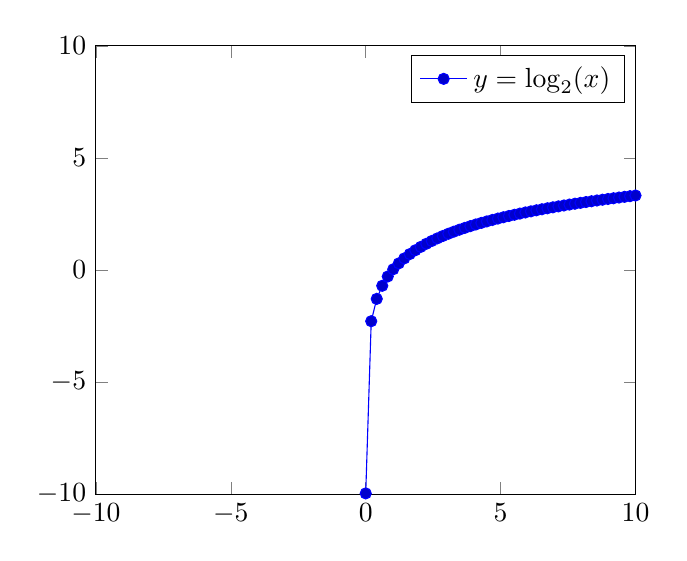
\begin{tikzpicture}
				\begin{axis}[
						xmin=-10,xmax=10,
						ymin=-10,ymax=10,
					]
					\addplot expression[domain=0.001:10,samples=50]{ln(x)/ln(2)};
					\addlegendentry{$y=\log_2(x)$}
				\end{axis}
			\end{tikzpicture}
			\item $b=\frac{1}{4}$
						
			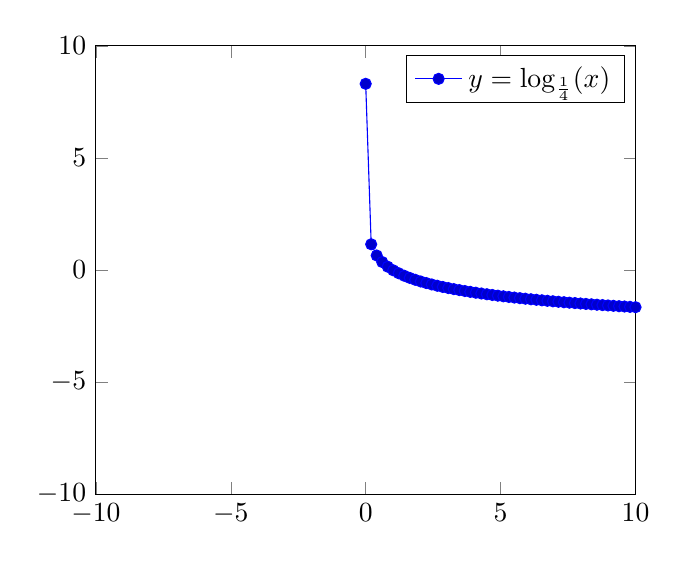
\begin{tikzpicture}
				\begin{axis}[
						xmin=-10,xmax=10,
						ymin=-10,ymax=10,
					]
					\addplot expression[domain=0.00001:10,samples=50]{ln(x)/ln(1/4)};
					\addlegendentry{$y=\log_{\frac{1}{4}}(x)$}
				\end{axis}
			\end{tikzpicture}
			\item $b=5$
						
			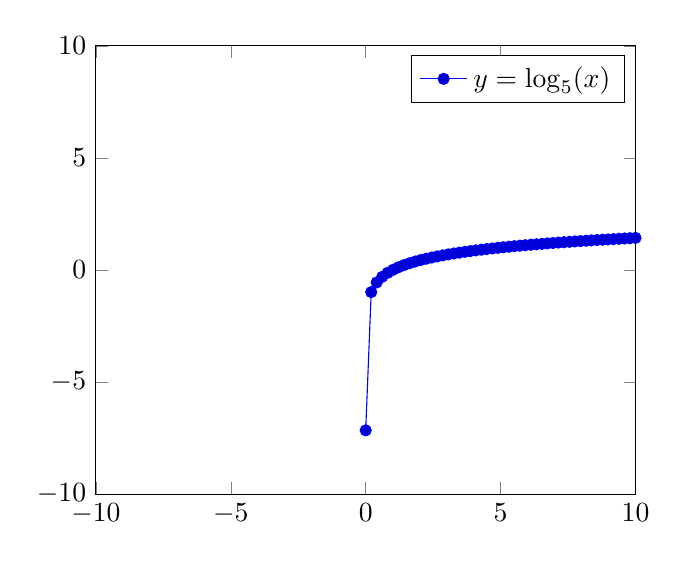
\begin{tikzpicture}
				\begin{axis}[
						xmin=-10,xmax=10,
						ymin=-10,ymax=10,
					]
					\addplot expression[domain=0.00001:10,samples=50]{ln(x)/ln(5)};
					\addlegendentry{$y=\log_5(x)$}
				\end{axis}
			\end{tikzpicture}
			\item $b=\frac{1}{3}$
						
			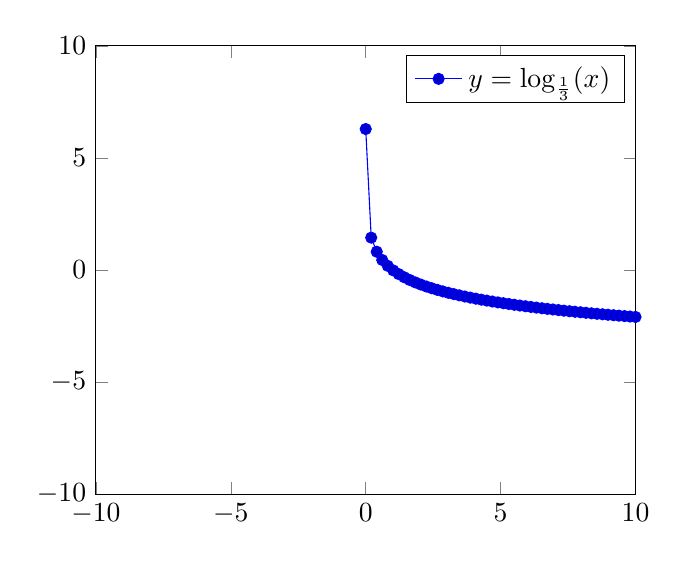
\begin{tikzpicture}
				\begin{axis}[
						xmin=-10,xmax=10,
						ymin=-10,ymax=10,
					]
					\addplot expression[domain=0.001:10,samples=50]{ln(x)/ln(1/3)};
					\addlegendentry{$y=\log_{\frac{1}{3}}(x)$}
				\end{axis}
			\end{tikzpicture}
		\end{enumerate}
	\end{shortsolution}
\end{subproblem}
Use your answer to \cref{log:prob:truefalse} to help you determine if 
each of the following statements are true or false for all values of $b$; if you believe that 
the statement is false, provide an example that supports it.
\begin{subproblem}
	The function $f$ is increasing.  
	\begin{shortsolution}
		False; consider $b=\frac{1}{4}$ or $b=\frac{1}{3}$, or any other value of $b$ such that $0<b<1$.
	\end{shortsolution}
\end{subproblem}
\begin{subproblem}
	The function $f$ is decreasing. 
	\begin{shortsolution}
		False; consider $b=2$ or $b=5$, or any other value of $b$ such that $b>1$.
	\end{shortsolution}
\end{subproblem}
\begin{subproblem}
	The function $f$ has a vertical asymptote at $0$. 
	\begin{shortsolution}
		True.
	\end{shortsolution}
\end{subproblem}
\begin{subproblem}
	The function $f$ is concave up.     
	\begin{shortsolution}
		False; consider $b=2$ or $b=5$, or any other value of $b$ such that $b>1$.
	\end{shortsolution}
\end{subproblem}
\begin{subproblem}
	The function $f$ has a zero at $1$. 
	\begin{shortsolution}
		True. 
	\end{shortsolution}
\end{subproblem}
\begin{subproblem}
	The function $f$ has a vertical intercept. 
	\begin{shortsolution}
		False; consider any value of $b$. 
	\end{shortsolution}
\end{subproblem}
\begin{subproblem}
	The function $f$ is concave down. 
	\begin{shortsolution}
		False; consider $b=\frac{1}{4}$ or $b=\frac{1}{3}$, or any other value of $b$ such that $0<b<1$.
	\end{shortsolution}
\end{subproblem}
\end{problem}

%===================================
%   Author: Hughes
%   Date:   July 2012
%===================================
\begin{problem}[\Cref{log:prop:add,log:prop:sub}]
\begin{subproblem}\label{log:prob:props}
	Use \cref{log:prop:add,log:prop:sub} to help you complete \cref{log:tab:props}; note that 
	you should be able to do so without using a calculator.
	\begin{shortsolution}
		\begin{tabular}[t]{S[table-format=2.3,parse-numbers=false]S[table-format=5.0,parse-numbers=false]S[table-format=1.0,parse-numbers=false]*{4}{S[table-format=1.0]}}
			\beforeheading
			\heading{$A$} & \heading{$B$}    & \heading{$b$}   & \heading{$\log_b(A)$} & \heading{$\log_b(B)$} & \heading{$\log_b(AB)$} & \heading{$\log_b\left( \frac{A}{B} \right)$} \\ 
			\afterheading
			1             & 2                & 2               & 0                     & 1                     & 1                      & -1                                           \\\normalline
			e^5           & e^3              & e               & 5                     & 3                     & 8                      & 2                                            \\\normalline
			36            & \sqrt[3]{6}      & 6               & 2                     & \num{1/3}             & \num{7/3}              & \num{5/3}                                    \\\normalline
			0.001         & 10000            & 10              & -3                    & 4                     & 1                      & -7                                           \\\normalline
			4             & \nicefrac{1}{16} & \nicefrac{1}{4} & -1                    & 2                     & 1                      & -3                                           \\\lastline
		\end{tabular}
	\end{shortsolution}
\end{subproblem}

\begin{table}[!htb]
	\centering
	\caption{\Cref{log:prop:add,log:prop:sub}}
	\label{log:tab:props}
	\begin{tabular}{S[table-format=2.3,parse-numbers=false]S[table-format=5.0,parse-numbers=false]S[table-format=2.0,parse-numbers=false]*{4}{c}}
		\beforeheading
		\heading{$A$} & \heading{$B$}    & \heading{$b$}   & \heading{$\log_b(A)$} & \heading{$\log_b(B)$} & \heading{$\log_b(AB)$} & \heading{$\log_b\left( \frac{A}{B} \right)$} \\ 
		\afterheading
		1             & 2                & 2               &                       &                       &                        &                                              \\\normalline
		e^5           & e^3              & e               &                       &                       &                        &                                              \\\normalline
		36            & \sqrt[3]{6}      & 6               &                       &                       &                        &                                              \\\normalline
		0.001         & 10000            & 10              &                       &                       &                        &                                              \\\normalline
		4             & \nicefrac{1}{16} & \nicefrac{1}{4} &                       &                       &                        &                                              \\\lastline
	\end{tabular}
\end{table}

Use your answer to \cref{log:prob:props} to help you decide if the following 
properties of logarithms are true or false.
\begin{subproblem}
	$\log_b(AB)=\log_b(A)\cdot\log_b(B)$    
	\begin{shortsolution}
		False.
	\end{shortsolution}
\end{subproblem}
\begin{subproblem}
	$\log_b(A+B)=\log_b(A)+\log_b(B)$ 
	\begin{shortsolution}
		False.
	\end{shortsolution}
\end{subproblem}
\begin{subproblem}
	$\log_b(AB)=\log_b(A)+\log_b(B)$ 
	\begin{shortsolution}
		True.
	\end{shortsolution}
\end{subproblem}
\begin{subproblem}
	$\log_b\left( \frac{A}{B} \right)=\frac{\log_b(A)}{\log_b(B)}$ 
	\begin{shortsolution}
		False.
	\end{shortsolution}
\end{subproblem}
\begin{subproblem}
	$\log_b\left( \frac{A}{B} \right)=\log_b(A)-\log_b(B)$
	\begin{shortsolution}
		True.
	\end{shortsolution}
\end{subproblem}
\end{problem}
\begin{exercises}
%===================================
%   Author: Hughes
%   Date:   July 2012
%===================================
\begin{problem}[Change of base]
Use the change of base formula, \cref{log:eq:changebase}, and a calculator to approximate each 
of the following (if possible).
\begin{multicols}{4}
	\begin{subproblem}
		$\log_2(3)$ 
		\begin{shortsolution}
			$\frac{\ln(3)}{\ln(2)}\approx 1.58$
		\end{shortsolution}
	\end{subproblem}
	\begin{subproblem}
		$\log_{23}(-2)$ 
		\begin{shortsolution}
			Undefined since the argument is negative. 
		\end{shortsolution}
	\end{subproblem}
	\begin{subproblem}
		$\log_3(7)$ 
		\begin{shortsolution}
			$\frac{\ln(7)}{\ln(3)}\approx 1.77$
		\end{shortsolution}
	\end{subproblem}
	\begin{subproblem}
		$\log_{\frac{1}{2}}(13)$ 
		\begin{shortsolution}
			$\frac{\ln(13)}{\ln\left( \frac{1}{2} \right)}\approx -3.70$
		\end{shortsolution}
	\end{subproblem}
	\begin{subproblem}
		$\log_8(2)$ 
		\begin{shortsolution}
			$\frac{\ln(2)}{\ln(8)}\approx .33$
		\end{shortsolution}
	\end{subproblem}
	\begin{subproblem}
		$\log_{-1}(5)$ 
		\begin{shortsolution}
			Undefined since the base is negative.
		\end{shortsolution}
	\end{subproblem}
	\begin{subproblem}
		$\log_\pi(5)$ 
		\begin{shortsolution}
			$\frac{\ln(5)}{\ln(\pi)}\approx 1.41$
		\end{shortsolution}
	\end{subproblem}
	\begin{subproblem}
		$\log_2(0)$ 
		\begin{shortsolution}
			Undefined since the argument is $0$.
		\end{shortsolution}
	\end{subproblem}
\end{multicols}
\end{problem}

%===================================
%   Author: Hughes
%   Date:   July 2012
%===================================
\begin{problem}[Expand logarithmic expressions]
Use the properties of logarithms to write each of the following 
expressions as the sum and/or difference of logarithms; leave
your answer in exact form.
\begin{multicols}{4}
	\begin{subproblem}
		$\log(2x)$ 
		\begin{shortsolution}
			$\log(2)+\log(x)$
		\end{shortsolution}
	\end{subproblem}
	\begin{subproblem}
		$\log_3\left( \frac{4}{x} \right)$ 
		\begin{shortsolution}
			$\log_3(4)-\log_3(x)$
		\end{shortsolution}
	\end{subproblem}
	\begin{subproblem}
		$\log_5(x^7)$ 
		\begin{shortsolution}
			$7\log_5(x)$ 
		\end{shortsolution}
	\end{subproblem}
	\begin{subproblem}
		$\log_9(4x^3)$ 
		\begin{shortsolution}
			$\log_9(4)+3\log_9(x)$
		\end{shortsolution}
	\end{subproblem}
	\begin{subproblem}
		$\ln(\sqrt{x})$ 
		\begin{shortsolution}
			$\frac{1}{2}\ln(x)$
		\end{shortsolution}
	\end{subproblem}
	\begin{subproblem}
		$\ln\left( \sqrt[7]{\frac{x^3}{x+2}} \right)$ 
		\begin{shortsolution}
			$\frac{3}{7}\ln(x)-\frac{1}{7}\ln(x+2)$
		\end{shortsolution}
	\end{subproblem}
	\begin{subproblem}
		$\log_\pi\left( \frac{x^2}{4} \right)$ 
		\begin{shortsolution}
			$2\log_\pi(x)-\log_\pi(4)$
		\end{shortsolution}
	\end{subproblem}
	\begin{subproblem}
		$3\log(10x)$ 
		\begin{shortsolution}
			$3+3\log(x)$
		\end{shortsolution}
	\end{subproblem}
\end{multicols}
\end{problem}

%===================================
%   Author: Hughes
%   Date:   July 2012
%===================================
\begin{problem}[Condense logarithmic expressions]
Use the properties of logarithms to write each of the following 
expressions as a single logarithm.
\fixthis{start and finish} 
\end{problem}

%===================================
%   Author: Hughes
%   Date:   July 2012
%===================================
\begin{problem}[Solving equations involving logarithms]
Use the properties of logarithms to help you solve the following 
equations.
\begin{multicols}{2} 
	\begin{subproblem}
		$\log_2(x)+\log_2(7)=3$ 
		\begin{shortsolution}
			$\frac{8}{7}$
		\end{shortsolution}
	\end{subproblem}
	\begin{subproblem}
		$\log_4(x)-\log_4(3)=-1$ 
		\begin{shortsolution}
			$\frac{3}{4}$ 
		\end{shortsolution}
	\end{subproblem}
	\begin{subproblem}
		$\log_3(x)+\log_3(9)=-2$ 
		\begin{shortsolution}
			$\frac{1}{81}$
		\end{shortsolution}
	\end{subproblem}
	\begin{subproblem}
		$\ln(2x)-\ln(9)=0$ 
		\begin{shortsolution}
			$\frac{9}{2}$
		\end{shortsolution}
	\end{subproblem}
\end{multicols}
\end{problem}
%===================================
%   Author: Hughes
%   Date:   July 2012
%===================================
\begin{problem}[Solving equations involving logarithms]
Use the properties of logarithms to help you solve the following 
equations.
\begin{multicols}{2}
	\begin{subproblem}
		$\log_2(x-2)+\log_2(x+9)=\log_2(12)$ 
		\begin{shortsolution}
			$3$
		\end{shortsolution}
	\end{subproblem}
	\begin{subproblem}
		$\ln(x+6)-\ln(x-2)=\ln(5)$ 
		\begin{shortsolution}
			$4$
		\end{shortsolution}
	\end{subproblem}
	\begin{subproblem}
		$\log(x+2)+\log(x-4)=\log(7)$ 
		\begin{shortsolution}
			$5$
		\end{shortsolution}
	\end{subproblem}
	\begin{subproblem}
		$\log_5(x+32)-\log_5(x)=\log_5(5)$ 
		\begin{shortsolution}
			$8$
		\end{shortsolution}
	\end{subproblem}
	\begin{subproblem}
		$\log_3(x-5)+\log_3(x)=\log_3(24)$ 
		\begin{shortsolution}
			$8$
		\end{shortsolution}
	\end{subproblem}
	\begin{subproblem}
		$\ln(x+76)-\ln(x+4)=\ln(9)$ 
		\begin{shortsolution}
			$5$
		\end{shortsolution}
	\end{subproblem}
	\begin{subproblem}
		$\log_{13}(x+3)+\log_{13}(x+1)=\log_{13}(24)$ 
		\begin{shortsolution}
			$3$
		\end{shortsolution}
	\end{subproblem}
	\begin{subproblem}
		$\log_{\pi}(x+58)-\log_{\pi}(x+7)=\log_{\pi}(4)$ 
		\begin{shortsolution}
			$10$
		\end{shortsolution}
	\end{subproblem}
\end{multicols}
\end{problem}

%===================================
%   Author: Hughes
%   Date:   July 2012
%===================================
\begin{problem}[Solving equations involving logarithms]
Use the properties of logarithms to help you solve the following 
equations.
\begin{multicols}{2}
	\begin{subproblem}
		$\log_2(x^2)+\log_2(7)=3$ 
		\begin{shortsolution}
			$\pm\frac{8}{7}$
		\end{shortsolution}
	\end{subproblem}
	\begin{subproblem}
		$\log(\sqrt[3]{x+1})+\log(x+1)=\log_2(16)$ 
		\begin{shortsolution}
			$999$
		\end{shortsolution}
	\end{subproblem}
	\begin{subproblem}
		$\log_3(\sqrt{x})-\log_3(5)=-2$ 
		\begin{shortsolution}
			$\frac{25}{81}$
		\end{shortsolution}
	\end{subproblem}
	\begin{subproblem}
		$\frac{1}{4}\ln(x+1) +\frac{1}{4}\ln(x)=1$
		\begin{shortsolution}
			$\frac{-1+\sqrt{1+4e^4}}{2}\approx 6.91$
		\end{shortsolution}
	\end{subproblem}
\end{multicols}
\end{problem}

%===================================
%   Author: Hughes
%   Date:   July 2012
%===================================
\begin{problem}[Piecewise logarithmic functions]
Consider the function $f$ that has formula
\[
	f(x)=
	\begin{cases}
		\log(x^2) & x <-2 \\
		\ln(x+2)  & x>-2  
	\end{cases}
\]
Evaluate each of the following (if possible), giving both the exact and an approximate answer.
\begin{multicols}{4}
	\begin{subproblem}
		$f(-5)$ 
		\begin{shortsolution}
			$\log(25)\approx 1.40$ 
		\end{shortsolution}
	\end{subproblem}
	\begin{subproblem}
		$f(-1)$ 
		\begin{shortsolution}
			$\ln(1)=0$ 
		\end{shortsolution}
	\end{subproblem}
	\begin{subproblem}
		$f(0)$ 
		\begin{shortsolution}
			$\ln(2)\approx 0.69$ 
		\end{shortsolution}
	\end{subproblem}
	\begin{subproblem}
		$f(-2)$ 
		\begin{shortsolution}
			Undefined. 
		\end{shortsolution}
	\end{subproblem}
\end{multicols}
\end{problem}

%===================================
%   Author: Hughes
%   Date:   July 2012
%===================================
\begin{problem}[Composition of logarithmic functions]
Let $f$ and $g$ be functions that have the following formulas
\[
	f(x)=\log(x+5), \qquad g(x)=\ln(x)
\]
Evaluate each of the following (if possible), giving both the exact 
and an approximate answer.
\begin{multicols}{4}
	\begin{subproblem}
		$(f\circ g)(1)$ 
		\begin{shortsolution}
			$\log(5)\approx 0.70$ 
		\end{shortsolution}
	\end{subproblem}
	\begin{subproblem}
		$(g\circ f)(1)$ 
		\begin{shortsolution}
			$-0.25$ 
		\end{shortsolution}
	\end{subproblem}
	\begin{subproblem}
		$\left(f\circ g \vphantom{e^{-5}}\right)\left( e^{-5} \right)$ 
		\begin{shortsolution}
			Undefined. 
		\end{shortsolution}
	\end{subproblem}
	\begin{subproblem}
		$(g\circ f)(-4)$ 
		\begin{shortsolution}
			Undefined. 
		\end{shortsolution}
	\end{subproblem}
	\begin{subproblem}
		$(f\circ g)\left( \frac{1}{2} \right)$ 
		\begin{shortsolution}
			$\log\left( \ln\left( \frac{1}{2} \right)+5 \right)\approx .63$ 
		\end{shortsolution}
	\end{subproblem}
	\begin{subproblem}
		$(f\circ g)(-3)$ 
		\begin{shortsolution}
			$\ln(\log(2))\approx -1.20$ 
		\end{shortsolution}
	\end{subproblem}
	\begin{subproblem}
		$(f\circ g)(x)$ 
		\begin{shortsolution}
			$\log(\ln(x)+5)$ 
		\end{shortsolution}
	\end{subproblem}
	\begin{subproblem}
		$(g\circ f)(x)$
		\begin{shortsolution}
			$\ln(\log(x+5))$ 
		\end{shortsolution}
	\end{subproblem}
\end{multicols}
\end{problem}

%===================================
%   Author: Hughes
%   Date:   August 2012
%===================================
\begin{problem}[Decomposition]
In each of the following problems, you are given a formula for function  
$h$. Decompose $h$ into two functions $f$ and $g$ such that $h=f\circ g$.
\begin{multicols}{4}
	\begin{subproblem}
		$h(x)=\log(3x^2)$
		\begin{shortsolution}
			$f(x)=\log(x)$, $g(x)=3x^2$
		\end{shortsolution}
	\end{subproblem}
	\begin{subproblem}
		$h(x)=-2\ln(5-x)$
		\begin{shortsolution}
			$f(x)=-2\ln(x)$, $g(x)=5-x$
		\end{shortsolution}
	\end{subproblem}
	\begin{subproblem}
		$h(x)=\log_3\left( \sqrt[3]{x} \right)$
		\begin{shortsolution}
			$f(x)=\log_3(x)$, $g(x)=\sqrt[3]{x}$
		\end{shortsolution}
	\end{subproblem}
	\begin{subproblem}
		$h(x)=\log_5(x^2)+7^{x^2}$
		\begin{shortsolution}
			$f(x)=\log_5(x)+7^x$, $g(x)=x^2$
		\end{shortsolution}
	\end{subproblem}
\end{multicols}
\end{problem}

%===================================
%   Author: Hughes
%   Date:   July 2012
%===================================
\begin{problem}[Function algebra]
Let $f$ and $g$ be the functions that have formulas
\[
	f(x)=\log(x), \qquad g(x)=\ln(x)
\]
Evaluate each of the following (if possible), giving the exact
and an approximate solution (where appropriate).
\begin{multicols}{4}
	\begin{subproblem}
		$(f+g)(1)$ 
		\begin{shortsolution}
			$2$ 
		\end{shortsolution}
	\end{subproblem}
	\begin{subproblem}
		$(f-g)(1)$ 
		\begin{shortsolution}
			$0$ 
		\end{shortsolution}
	\end{subproblem}
	\begin{subproblem}
		$(f\cdot g)(1)$ 
		\begin{shortsolution}
			$1$ 
		\end{shortsolution}
	\end{subproblem}
	\begin{subproblem}
		$\left( \frac{f}{g} \right)(1)$ 
		\begin{shortsolution}
			Undefined. 
		\end{shortsolution}
	\end{subproblem}
	\begin{subproblem}
		$(f+g)(5)$ 
		\begin{shortsolution}
			$\log(5)+\ln(5)\approx 2.31$ 
		\end{shortsolution}
	\end{subproblem}
	\begin{subproblem}
		$(f-g)(\pi)$ 
		\begin{shortsolution}
			$\log(\pi)-\ln(\pi)\approx -0.65$       
		\end{shortsolution}
	\end{subproblem}
	\begin{subproblem}
		$(f\cdot g)(e)$ 
		\begin{shortsolution}
			$\log(e)\approx .43$  
		\end{shortsolution}
	\end{subproblem}
	\begin{subproblem}
		$\left( \frac{f}{g} \right)\left( \frac{1}{2} \right)$ 
		\begin{shortsolution}
			$\frac{\log\left( \frac{1}{2} \right)}{\ln\left( \frac{1}{2} \right)}\approx 0.43$ 
		\end{shortsolution}
	\end{subproblem}
\end{multicols}
\end{problem}

\end{exercises}
